% Graphic for TeX using PGF
% Title: /home/satenske/cours/OMGL/prl3/TD3/diag4.dia
% Creator: Dia v0.97.1
% CreationDate: Mon Oct  3 22:14:40 2011
% For: satenske
% \usepackage{tikz}
% The following commands are not supported in PSTricks at present
% We define them conditionally, so when they are implemented,
% this pgf file will use them.
\ifx\du\undefined
  \newlength{\du}
\fi
\setlength{\du}{15\unitlength}
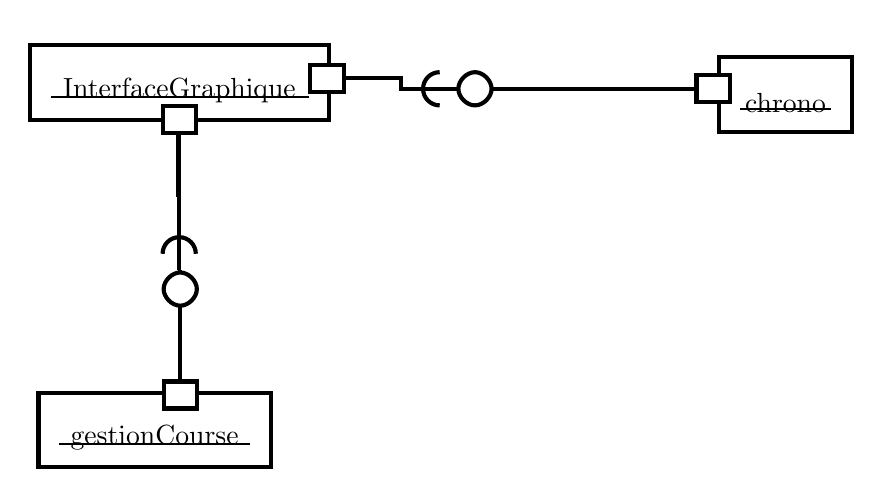
\begin{tikzpicture}
\pgftransformxscale{1.000000}
\pgftransformyscale{-1.000000}
\definecolor{dialinecolor}{rgb}{0.000000, 0.000000, 0.000000}
\pgfsetstrokecolor{dialinecolor}
\definecolor{dialinecolor}{rgb}{1.000000, 1.000000, 1.000000}
\pgfsetfillcolor{dialinecolor}
\pgfsetlinewidth{0.100000\du}
\pgfsetdash{}{0pt}
\definecolor{dialinecolor}{rgb}{1.000000, 1.000000, 1.000000}
\pgfsetfillcolor{dialinecolor}
\fill (20.400000\du,6.850000\du)--(20.400000\du,8.650000\du)--(27.615000\du,8.650000\du)--(27.615000\du,6.850000\du)--cycle;
\definecolor{dialinecolor}{rgb}{0.000000, 0.000000, 0.000000}
\pgfsetstrokecolor{dialinecolor}
\draw (20.400000\du,6.850000\du)--(20.400000\du,8.650000\du)--(27.615000\du,8.650000\du)--(27.615000\du,6.850000\du)--cycle;
% setfont left to latex
\definecolor{dialinecolor}{rgb}{0.000000, 0.000000, 0.000000}
\pgfsetstrokecolor{dialinecolor}
\node at (24.007500\du,7.945000\du){InterfaceGraphique};
% setfont left to latex
\pgfsetlinewidth{0.050000\du}
\definecolor{dialinecolor}{rgb}{0.000000, 0.000000, 0.000000}
\pgfsetstrokecolor{dialinecolor}
\draw (20.900000\du,8.097500\du)--(27.115000\du,8.097500\du);
\pgfsetlinewidth{0.100000\du}
\pgfsetdash{}{0pt}
\definecolor{dialinecolor}{rgb}{1.000000, 1.000000, 1.000000}
\pgfsetfillcolor{dialinecolor}
\fill (20.610000\du,15.220000\du)--(20.610000\du,17.020000\du)--(26.205000\du,17.020000\du)--(26.205000\du,15.220000\du)--cycle;
\definecolor{dialinecolor}{rgb}{0.000000, 0.000000, 0.000000}
\pgfsetstrokecolor{dialinecolor}
\draw (20.610000\du,15.220000\du)--(20.610000\du,17.020000\du)--(26.205000\du,17.020000\du)--(26.205000\du,15.220000\du)--cycle;
% setfont left to latex
\definecolor{dialinecolor}{rgb}{0.000000, 0.000000, 0.000000}
\pgfsetstrokecolor{dialinecolor}
\node at (23.407500\du,16.315000\du){gestionCourse};
% setfont left to latex
\pgfsetlinewidth{0.050000\du}
\definecolor{dialinecolor}{rgb}{0.000000, 0.000000, 0.000000}
\pgfsetstrokecolor{dialinecolor}
\draw (21.110000\du,16.467500\du)--(25.705000\du,16.467500\du);
\pgfsetlinewidth{0.100000\du}
\pgfsetdash{}{0pt}
\pgfsetbuttcap
{
\definecolor{dialinecolor}{rgb}{0.000000, 0.000000, 0.000000}
\pgfsetfillcolor{dialinecolor}
% was here!!!
\definecolor{dialinecolor}{rgb}{0.000000, 0.000000, 0.000000}
\pgfsetstrokecolor{dialinecolor}
\draw (23.982500\du,8.650000\du)--(23.982500\du,10.462500\du)--(24.000000\du,10.462500\du)--(24.000000\du,12.275000\du);
}
\definecolor{dialinecolor}{rgb}{0.000000, 0.000000, 0.000000}
\pgfsetstrokecolor{dialinecolor}
\draw (23.982500\du,8.650000\du)--(23.982500\du,10.462500\du)--(24.000000\du,10.462500\du)--(24.000000\du,11.475000\du);
\pgfsetdash{}{0pt}
\pgfsetmiterjoin
\pgfsetbuttcap
\pgfsetlinewidth{0.100000\du}
\definecolor{dialinecolor}{rgb}{0.000000, 0.000000, 0.000000}
\pgfsetstrokecolor{dialinecolor}
\pgfpathmoveto{\pgfpoint{24.400000\du}{11.874681\du}}
\pgfpatharc{360}{180}{0.400000\du and 0.400000\du}
\pgfusepath{stroke}
% setfont left to latex
\definecolor{dialinecolor}{rgb}{0.000000, 0.000000, 0.000000}
\pgfsetstrokecolor{dialinecolor}
\node at (23.900000\du,6.800000\du){};
\pgfsetlinewidth{0.100000\du}
\pgfsetdash{}{0pt}
\pgfsetbuttcap
{
\definecolor{dialinecolor}{rgb}{0.000000, 0.000000, 0.000000}
\pgfsetfillcolor{dialinecolor}
% was here!!!
\definecolor{dialinecolor}{rgb}{0.000000, 0.000000, 0.000000}
\pgfsetstrokecolor{dialinecolor}
\draw (24.025000\du,14.899634\du)--(24.025000\du,14.899634\du)--(24.025000\du,12.275000\du)--(24.025000\du,12.275000\du);
}
\definecolor{dialinecolor}{rgb}{0.000000, 0.000000, 0.000000}
\pgfsetstrokecolor{dialinecolor}
\draw (24.025000\du,14.899634\du)--(24.025000\du,14.899634\du)--(24.025000\du,13.125000\du);
\pgfsetlinewidth{0.100000\du}
\pgfsetdash{}{0pt}
\pgfsetmiterjoin
\pgfsetbuttcap
\definecolor{dialinecolor}{rgb}{1.000000, 1.000000, 1.000000}
\pgfsetfillcolor{dialinecolor}
\pgfpathmoveto{\pgfpoint{24.025000\du}{12.325000\du}}
\pgfpathcurveto{\pgfpoint{24.225000\du}{12.325000\du}}{\pgfpoint{24.425000\du}{12.525000\du}}{\pgfpoint{24.425000\du}{12.725000\du}}
\pgfpathcurveto{\pgfpoint{24.425000\du}{12.925000\du}}{\pgfpoint{24.225000\du}{13.125000\du}}{\pgfpoint{24.025000\du}{13.125000\du}}
\pgfpathcurveto{\pgfpoint{23.825000\du}{13.125000\du}}{\pgfpoint{23.625000\du}{12.925000\du}}{\pgfpoint{23.625000\du}{12.725000\du}}
\pgfpathcurveto{\pgfpoint{23.625000\du}{12.525000\du}}{\pgfpoint{23.825000\du}{12.325000\du}}{\pgfpoint{24.025000\du}{12.325000\du}}
\pgfusepath{fill}
\definecolor{dialinecolor}{rgb}{0.000000, 0.000000, 0.000000}
\pgfsetstrokecolor{dialinecolor}
\pgfpathmoveto{\pgfpoint{24.025000\du}{12.325000\du}}
\pgfpathcurveto{\pgfpoint{24.225000\du}{12.325000\du}}{\pgfpoint{24.425000\du}{12.525000\du}}{\pgfpoint{24.425000\du}{12.725000\du}}
\pgfpathcurveto{\pgfpoint{24.425000\du}{12.925000\du}}{\pgfpoint{24.225000\du}{13.125000\du}}{\pgfpoint{24.025000\du}{13.125000\du}}
\pgfpathcurveto{\pgfpoint{23.825000\du}{13.125000\du}}{\pgfpoint{23.625000\du}{12.925000\du}}{\pgfpoint{23.625000\du}{12.725000\du}}
\pgfpathcurveto{\pgfpoint{23.625000\du}{12.525000\du}}{\pgfpoint{23.825000\du}{12.325000\du}}{\pgfpoint{24.025000\du}{12.325000\du}}
\pgfusepath{stroke}
% setfont left to latex
\definecolor{dialinecolor}{rgb}{0.000000, 0.000000, 0.000000}
\pgfsetstrokecolor{dialinecolor}
\node at (24.025000\du,15.175000\du){};
\pgfsetlinewidth{0.100000\du}
\pgfsetdash{}{0pt}
\pgfsetdash{}{0pt}
\pgfsetmiterjoin
\definecolor{dialinecolor}{rgb}{1.000000, 1.000000, 1.000000}
\pgfsetfillcolor{dialinecolor}
\fill (23.625000\du,14.950000\du)--(23.625000\du,15.600000\du)--(24.425000\du,15.600000\du)--(24.425000\du,14.950000\du)--cycle;
\definecolor{dialinecolor}{rgb}{0.000000, 0.000000, 0.000000}
\pgfsetstrokecolor{dialinecolor}
\draw (23.625000\du,14.950000\du)--(23.625000\du,15.600000\du)--(24.425000\du,15.600000\du)--(24.425000\du,14.950000\du)--cycle;
\pgfsetlinewidth{0.100000\du}
\pgfsetdash{}{0pt}
\pgfsetdash{}{0pt}
\pgfsetmiterjoin
\definecolor{dialinecolor}{rgb}{1.000000, 1.000000, 1.000000}
\pgfsetfillcolor{dialinecolor}
\fill (23.610000\du,8.320000\du)--(23.610000\du,8.970000\du)--(24.410000\du,8.970000\du)--(24.410000\du,8.320000\du)--cycle;
\definecolor{dialinecolor}{rgb}{0.000000, 0.000000, 0.000000}
\pgfsetstrokecolor{dialinecolor}
\draw (23.610000\du,8.320000\du)--(23.610000\du,8.970000\du)--(24.410000\du,8.970000\du)--(24.410000\du,8.320000\du)--cycle;
\pgfsetlinewidth{0.100000\du}
\pgfsetdash{}{0pt}
\pgfsetdash{}{0pt}
\pgfsetmiterjoin
\definecolor{dialinecolor}{rgb}{1.000000, 1.000000, 1.000000}
\pgfsetfillcolor{dialinecolor}
\fill (27.160000\du,7.320000\du)--(27.160000\du,7.970000\du)--(27.960000\du,7.970000\du)--(27.960000\du,7.320000\du)--cycle;
\definecolor{dialinecolor}{rgb}{0.000000, 0.000000, 0.000000}
\pgfsetstrokecolor{dialinecolor}
\draw (27.160000\du,7.320000\du)--(27.160000\du,7.970000\du)--(27.960000\du,7.970000\du)--(27.960000\du,7.320000\du)--cycle;
\pgfsetlinewidth{0.100000\du}
\pgfsetdash{}{0pt}
\definecolor{dialinecolor}{rgb}{1.000000, 1.000000, 1.000000}
\pgfsetfillcolor{dialinecolor}
\fill (37.010000\du,7.140000\du)--(37.010000\du,8.940000\du)--(40.205000\du,8.940000\du)--(40.205000\du,7.140000\du)--cycle;
\definecolor{dialinecolor}{rgb}{0.000000, 0.000000, 0.000000}
\pgfsetstrokecolor{dialinecolor}
\draw (37.010000\du,7.140000\du)--(37.010000\du,8.940000\du)--(40.205000\du,8.940000\du)--(40.205000\du,7.140000\du)--cycle;
% setfont left to latex
\definecolor{dialinecolor}{rgb}{0.000000, 0.000000, 0.000000}
\pgfsetstrokecolor{dialinecolor}
\node at (38.607500\du,8.235000\du){chrono};
% setfont left to latex
\pgfsetlinewidth{0.050000\du}
\definecolor{dialinecolor}{rgb}{0.000000, 0.000000, 0.000000}
\pgfsetstrokecolor{dialinecolor}
\draw (37.510000\du,8.387500\du)--(39.705000\du,8.387500\du);
\pgfsetlinewidth{0.100000\du}
\pgfsetdash{}{0pt}
\pgfsetbuttcap
{
\definecolor{dialinecolor}{rgb}{0.000000, 0.000000, 0.000000}
\pgfsetfillcolor{dialinecolor}
% was here!!!
\definecolor{dialinecolor}{rgb}{0.000000, 0.000000, 0.000000}
\pgfsetstrokecolor{dialinecolor}
\draw (36.409561\du,7.895000\du)--(33.542280\du,7.895000\du)--(33.542280\du,7.900000\du)--(30.675000\du,7.900000\du);
}
\definecolor{dialinecolor}{rgb}{0.000000, 0.000000, 0.000000}
\pgfsetstrokecolor{dialinecolor}
\draw (36.409561\du,7.895000\du)--(33.542280\du,7.895000\du)--(33.542280\du,7.900000\du)--(31.525000\du,7.900000\du);
\pgfsetlinewidth{0.100000\du}
\pgfsetdash{}{0pt}
\pgfsetmiterjoin
\pgfsetbuttcap
\definecolor{dialinecolor}{rgb}{1.000000, 1.000000, 1.000000}
\pgfsetfillcolor{dialinecolor}
\pgfpathmoveto{\pgfpoint{30.725000\du}{7.900000\du}}
\pgfpathcurveto{\pgfpoint{30.725000\du}{7.700000\du}}{\pgfpoint{30.925000\du}{7.500000\du}}{\pgfpoint{31.125000\du}{7.500000\du}}
\pgfpathcurveto{\pgfpoint{31.325000\du}{7.500000\du}}{\pgfpoint{31.525000\du}{7.700000\du}}{\pgfpoint{31.525000\du}{7.900000\du}}
\pgfpathcurveto{\pgfpoint{31.525000\du}{8.100000\du}}{\pgfpoint{31.325000\du}{8.300000\du}}{\pgfpoint{31.125000\du}{8.300000\du}}
\pgfpathcurveto{\pgfpoint{30.925000\du}{8.300000\du}}{\pgfpoint{30.725000\du}{8.100000\du}}{\pgfpoint{30.725000\du}{7.900000\du}}
\pgfusepath{fill}
\definecolor{dialinecolor}{rgb}{0.000000, 0.000000, 0.000000}
\pgfsetstrokecolor{dialinecolor}
\pgfpathmoveto{\pgfpoint{30.725000\du}{7.900000\du}}
\pgfpathcurveto{\pgfpoint{30.725000\du}{7.700000\du}}{\pgfpoint{30.925000\du}{7.500000\du}}{\pgfpoint{31.125000\du}{7.500000\du}}
\pgfpathcurveto{\pgfpoint{31.325000\du}{7.500000\du}}{\pgfpoint{31.525000\du}{7.700000\du}}{\pgfpoint{31.525000\du}{7.900000\du}}
\pgfpathcurveto{\pgfpoint{31.525000\du}{8.100000\du}}{\pgfpoint{31.325000\du}{8.300000\du}}{\pgfpoint{31.125000\du}{8.300000\du}}
\pgfpathcurveto{\pgfpoint{30.925000\du}{8.300000\du}}{\pgfpoint{30.725000\du}{8.100000\du}}{\pgfpoint{30.725000\du}{7.900000\du}}
\pgfusepath{stroke}
% setfont left to latex
\definecolor{dialinecolor}{rgb}{0.000000, 0.000000, 0.000000}
\pgfsetstrokecolor{dialinecolor}
\node at (37.300000\du,7.470000\du){};
\pgfsetlinewidth{0.100000\du}
\pgfsetdash{}{0pt}
\pgfsetbuttcap
{
\definecolor{dialinecolor}{rgb}{0.000000, 0.000000, 0.000000}
\pgfsetfillcolor{dialinecolor}
% was here!!!
\definecolor{dialinecolor}{rgb}{0.000000, 0.000000, 0.000000}
\pgfsetstrokecolor{dialinecolor}
\draw (28.010439\du,7.645000\du)--(29.342720\du,7.645000\du)--(29.342720\du,7.900000\du)--(30.675000\du,7.900000\du);
}
\definecolor{dialinecolor}{rgb}{0.000000, 0.000000, 0.000000}
\pgfsetstrokecolor{dialinecolor}
\draw (28.010439\du,7.645000\du)--(29.342720\du,7.645000\du)--(29.342720\du,7.900000\du)--(29.875000\du,7.900000\du);
\pgfsetdash{}{0pt}
\pgfsetmiterjoin
\pgfsetbuttcap
\pgfsetlinewidth{0.100000\du}
\definecolor{dialinecolor}{rgb}{0.000000, 0.000000, 0.000000}
\pgfsetstrokecolor{dialinecolor}
\pgfpathmoveto{\pgfpoint{30.275011\du}{7.500000\du}}
\pgfpatharc{270}{90}{0.400000\du and 0.400000\du}
\pgfusepath{stroke}
% setfont left to latex
\definecolor{dialinecolor}{rgb}{0.000000, 0.000000, 0.000000}
\pgfsetstrokecolor{dialinecolor}
\node at (27.650000\du,6.650000\du){};
\pgfsetlinewidth{0.100000\du}
\pgfsetdash{}{0pt}
\pgfsetdash{}{0pt}
\pgfsetmiterjoin
\definecolor{dialinecolor}{rgb}{1.000000, 1.000000, 1.000000}
\pgfsetfillcolor{dialinecolor}
\fill (36.460000\du,7.570000\du)--(36.460000\du,8.220000\du)--(37.260000\du,8.220000\du)--(37.260000\du,7.570000\du)--cycle;
\definecolor{dialinecolor}{rgb}{0.000000, 0.000000, 0.000000}
\pgfsetstrokecolor{dialinecolor}
\draw (36.460000\du,7.570000\du)--(36.460000\du,8.220000\du)--(37.260000\du,8.220000\du)--(37.260000\du,7.570000\du)--cycle;
\end{tikzpicture}
